\documentclass[twoside]{book}

% Packages required by doxygen
\usepackage{fixltx2e}
\usepackage{calc}
\usepackage{doxygen}
\usepackage[export]{adjustbox} % also loads graphicx
\usepackage{graphicx}
\usepackage[utf8]{inputenc}
\usepackage{makeidx}
\usepackage{multicol}
\usepackage{multirow}
\PassOptionsToPackage{warn}{textcomp}
\usepackage{textcomp}
\usepackage[nointegrals]{wasysym}
\usepackage[table]{xcolor}

% NLS support packages
\usepackage[T2A]{fontenc}
\usepackage[russian]{babel}

% Font selection
\usepackage[T1]{fontenc}
\usepackage[scaled=.90]{helvet}
\usepackage{courier}
\usepackage{amssymb}
\usepackage{sectsty}
\renewcommand{\familydefault}{\sfdefault}
\allsectionsfont{%
  \fontseries{bc}\selectfont%
  \color{darkgray}%
}
\renewcommand{\DoxyLabelFont}{%
  \fontseries{bc}\selectfont%
  \color{darkgray}%
}
\newcommand{\+}{\discretionary{\mbox{\scriptsize$\hookleftarrow$}}{}{}}

% Page & text layout
\usepackage{geometry}
\geometry{%
  a4paper,%
  top=2.5cm,%
  bottom=2.5cm,%
  left=2.5cm,%
  right=2.5cm%
}
\tolerance=750
\hfuzz=15pt
\hbadness=750
\setlength{\emergencystretch}{15pt}
\setlength{\parindent}{0cm}
\setlength{\parskip}{3ex plus 2ex minus 2ex}
\makeatletter
\renewcommand{\paragraph}{%
  \@startsection{paragraph}{4}{0ex}{-1.0ex}{1.0ex}{%
    \normalfont\normalsize\bfseries\SS@parafont%
  }%
}
\renewcommand{\subparagraph}{%
  \@startsection{subparagraph}{5}{0ex}{-1.0ex}{1.0ex}{%
    \normalfont\normalsize\bfseries\SS@subparafont%
  }%
}
\makeatother

% Headers & footers
\usepackage{fancyhdr}
\pagestyle{fancyplain}
\fancyhead[LE]{\fancyplain{}{\bfseries\thepage}}
\fancyhead[CE]{\fancyplain{}{}}
\fancyhead[RE]{\fancyplain{}{\bfseries\leftmark}}
\fancyhead[LO]{\fancyplain{}{\bfseries\rightmark}}
\fancyhead[CO]{\fancyplain{}{}}
\fancyhead[RO]{\fancyplain{}{\bfseries\thepage}}
\fancyfoot[LE]{\fancyplain{}{}}
\fancyfoot[CE]{\fancyplain{}{}}
\fancyfoot[RE]{\fancyplain{}{\bfseries\scriptsize Создано системой Doxygen }}
\fancyfoot[LO]{\fancyplain{}{\bfseries\scriptsize Создано системой Doxygen }}
\fancyfoot[CO]{\fancyplain{}{}}
\fancyfoot[RO]{\fancyplain{}{}}
\renewcommand{\footrulewidth}{0.4pt}
\renewcommand{\chaptermark}[1]{%
  \markboth{#1}{}%
}
\renewcommand{\sectionmark}[1]{%
  \markright{\thesection\ #1}%
}

% Indices & bibliography
\usepackage{natbib}
\usepackage[titles]{tocloft}
\setcounter{tocdepth}{3}
\setcounter{secnumdepth}{5}
\makeindex

% Hyperlinks (required, but should be loaded last)
\usepackage{ifpdf}
\ifpdf
  \usepackage[pdftex,pagebackref=true]{hyperref}
\else
  \usepackage[ps2pdf,pagebackref=true]{hyperref}
\fi
\hypersetup{%
  colorlinks=true,%
  linkcolor=blue,%
  citecolor=blue,%
  unicode%
}

% Custom commands
\newcommand{\clearemptydoublepage}{%
  \newpage{\pagestyle{empty}\cleardoublepage}%
}

\usepackage{caption}
\captionsetup{labelsep=space,justification=centering,font={bf},singlelinecheck=off,skip=4pt,position=top}

%===== C O N T E N T S =====

\begin{document}

% Titlepage & ToC
\hypersetup{pageanchor=false,
             bookmarksnumbered=true,
             pdfencoding=unicode
            }
\pagenumbering{alph}
\begin{titlepage}
\vspace*{7cm}
\begin{center}%
{\Large Galois\+\_\+\+L\+F\+SR \\[1ex]\large 1.\+0.\+0 }\\
\vspace*{1cm}
{\large Создано системой Doxygen 1.8.13}\\
\end{center}
\end{titlepage}
\clearemptydoublepage
\pagenumbering{roman}
\tableofcontents
\clearemptydoublepage
\pagenumbering{arabic}
\hypersetup{pageanchor=true}

%--- Begin generated contents ---
\chapter{Иерархический список классов}
\section{Иерархия классов}
Иерархия классов.\begin{DoxyCompactList}
\item \contentsline{section}{Galois\+\_\+\+L\+F\+SR}{\pageref{classGalois__LFSR}}{}
\item runtime\+\_\+error\begin{DoxyCompactList}
\item \contentsline{section}{Galois\+Error}{\pageref{classGaloisError}}{}
\end{DoxyCompactList}
\end{DoxyCompactList}

\chapter{Алфавитный указатель классов}
\section{Классы}
Классы с их кратким описанием.\begin{DoxyCompactList}
\item\contentsline{section}{\hyperlink{classGalois__LFSR}{Galois\+\_\+\+L\+F\+SR} }{\pageref{classGalois__LFSR}}{}
\item\contentsline{section}{\hyperlink{classGaloisError}{Galois\+Error} \\*Класс-\/исключение }{\pageref{classGaloisError}}{}
\end{DoxyCompactList}

\chapter{Список файлов}
\section{Файлы}
Полный список документированных файлов.\begin{DoxyCompactList}
\item\contentsline{section}{\hyperlink{Galois__LFSR_8cpp}{Galois\+\_\+\+L\+F\+S\+R.\+cpp} \\*Конструктор по-\/умолчанию, не принимает ничего на вход }{\pageref{Galois__LFSR_8cpp}}{}
\item\contentsline{section}{\hyperlink{Galois__LFSR_8h}{Galois\+\_\+\+L\+F\+S\+R.\+h} \\*Программа генерации псевдослучайно последовательности на базе регистра сдвига с линейной обратной связью с разрядностью 48 бит в конфигурации Галуа }{\pageref{Galois__LFSR_8h}}{}
\item\contentsline{section}{\hyperlink{main_8cpp}{main.\+cpp} }{\pageref{main_8cpp}}{}
\end{DoxyCompactList}

\chapter{Классы}
\hypertarget{classGalois__LFSR}{}\section{Класс Galois\+\_\+\+L\+F\+SR}
\label{classGalois__LFSR}\index{Galois\+\_\+\+L\+F\+SR@{Galois\+\_\+\+L\+F\+SR}}


{\ttfamily \#include $<$Galois\+\_\+\+L\+F\+S\+R.\+h$>$}

\subsection*{Открытые члены}
\begin{DoxyCompactItemize}
\item 
\mbox{\Hypertarget{classGalois__LFSR_a23455fca80e4ed521062a7b2842edb03}\label{classGalois__LFSR_a23455fca80e4ed521062a7b2842edb03}} 
\hyperlink{classGalois__LFSR_a23455fca80e4ed521062a7b2842edb03}{Galois\+\_\+\+L\+F\+SR} ()
\begin{DoxyCompactList}\small\item\em Конструктор \end{DoxyCompactList}\item 
void \hyperlink{classGalois__LFSR_a7a2d2fa3f9f7973cb520d92267f58f4d}{print\+\_\+bits} (uint64\+\_\+t bits)
\begin{DoxyCompactList}\small\item\em Функция для вывода числа в битном представлении \end{DoxyCompactList}\item 
void \hyperlink{classGalois__LFSR_aa3a893992b929b01a649d859a121ae34}{set\+\_\+start\+\_\+bits} (uint64\+\_\+t bits)
\begin{DoxyCompactList}\small\item\em Функция для установки начальной позиции \end{DoxyCompactList}\item 
uint64\+\_\+t \hyperlink{classGalois__LFSR_aea6f1eea9ba930bb7419426a45a59c5c}{get\+\_\+start\+\_\+bits} ()
\begin{DoxyCompactList}\small\item\em Функция возвращает начальное значение \end{DoxyCompactList}\item 
uint64\+\_\+t \hyperlink{classGalois__LFSR_abc5cfd0aa22803188a1f81a5959f22eb}{get\+\_\+random\+\_\+bits} ()
\begin{DoxyCompactList}\small\item\em Функция для генерации случайной начальной позиции \end{DoxyCompactList}\item 
uint64\+\_\+t \hyperlink{classGalois__LFSR_ae8b9c21348f0f6f75c539e7a8667be88}{reverse\+\_\+bits} (uint64\+\_\+t bits)
\begin{DoxyCompactList}\small\item\em Функция для нахождения перевёрнутого числа \end{DoxyCompactList}\item 
uint64\+\_\+t \hyperlink{classGalois__LFSR_a1ceda4d66d840ff703cd14a3919b2f8b}{get\+\_\+respond\+\_\+bits} (bool is\+\_\+random\+\_\+bits)
\begin{DoxyCompactList}\small\item\em Функция для генерации псевдослучайного числа \end{DoxyCompactList}\end{DoxyCompactItemize}


\subsection{Подробное описание}
\begin{DoxyAuthor}{Автор}
vo5torg 
\end{DoxyAuthor}
\begin{DoxyDate}{Дата}
06/22/21 
\end{DoxyDate}


\subsection{Методы}
\mbox{\Hypertarget{classGalois__LFSR_abc5cfd0aa22803188a1f81a5959f22eb}\label{classGalois__LFSR_abc5cfd0aa22803188a1f81a5959f22eb}} 
\index{Galois\+\_\+\+L\+F\+SR@{Galois\+\_\+\+L\+F\+SR}!get\+\_\+random\+\_\+bits@{get\+\_\+random\+\_\+bits}}
\index{get\+\_\+random\+\_\+bits@{get\+\_\+random\+\_\+bits}!Galois\+\_\+\+L\+F\+SR@{Galois\+\_\+\+L\+F\+SR}}
\subsubsection{\texorpdfstring{get\+\_\+random\+\_\+bits()}{get\_random\_bits()}}
{\footnotesize\ttfamily uint64\+\_\+t Galois\+\_\+\+L\+F\+S\+R\+::get\+\_\+random\+\_\+bits (\begin{DoxyParamCaption}{ }\end{DoxyParamCaption})}



Функция для генерации случайной начальной позиции 

Функция генерирует случайное число.

\begin{DoxyReturn}{Возвращает}
Случайное число 
\end{DoxyReturn}
\mbox{\Hypertarget{classGalois__LFSR_a1ceda4d66d840ff703cd14a3919b2f8b}\label{classGalois__LFSR_a1ceda4d66d840ff703cd14a3919b2f8b}} 
\index{Galois\+\_\+\+L\+F\+SR@{Galois\+\_\+\+L\+F\+SR}!get\+\_\+respond\+\_\+bits@{get\+\_\+respond\+\_\+bits}}
\index{get\+\_\+respond\+\_\+bits@{get\+\_\+respond\+\_\+bits}!Galois\+\_\+\+L\+F\+SR@{Galois\+\_\+\+L\+F\+SR}}
\subsubsection{\texorpdfstring{get\+\_\+respond\+\_\+bits()}{get\_respond\_bits()}}
{\footnotesize\ttfamily uint64\+\_\+t Galois\+\_\+\+L\+F\+S\+R\+::get\+\_\+respond\+\_\+bits (\begin{DoxyParamCaption}\item[{bool}]{is\+\_\+random\+\_\+bits }\end{DoxyParamCaption})}



Функция для генерации псевдослучайного числа 

Функция принимает на вход булеву переменную. Генерирует псевдослучайное число.


\begin{DoxyParams}{Аргументы}
{\em is\+\_\+random\+\_\+bits} & \\
\hline
\end{DoxyParams}
\begin{DoxyReturn}{Возвращает}
Псевдослучайное число 
\end{DoxyReturn}
\mbox{\Hypertarget{classGalois__LFSR_aea6f1eea9ba930bb7419426a45a59c5c}\label{classGalois__LFSR_aea6f1eea9ba930bb7419426a45a59c5c}} 
\index{Galois\+\_\+\+L\+F\+SR@{Galois\+\_\+\+L\+F\+SR}!get\+\_\+start\+\_\+bits@{get\+\_\+start\+\_\+bits}}
\index{get\+\_\+start\+\_\+bits@{get\+\_\+start\+\_\+bits}!Galois\+\_\+\+L\+F\+SR@{Galois\+\_\+\+L\+F\+SR}}
\subsubsection{\texorpdfstring{get\+\_\+start\+\_\+bits()}{get\_start\_bits()}}
{\footnotesize\ttfamily uint64\+\_\+t Galois\+\_\+\+L\+F\+S\+R\+::get\+\_\+start\+\_\+bits (\begin{DoxyParamCaption}{ }\end{DoxyParamCaption})}



Функция возвращает начальное значение 

Функция возвращает начальный регистр.

\begin{DoxyReturn}{Возвращает}
Начальный регистр 
\end{DoxyReturn}
\mbox{\Hypertarget{classGalois__LFSR_a7a2d2fa3f9f7973cb520d92267f58f4d}\label{classGalois__LFSR_a7a2d2fa3f9f7973cb520d92267f58f4d}} 
\index{Galois\+\_\+\+L\+F\+SR@{Galois\+\_\+\+L\+F\+SR}!print\+\_\+bits@{print\+\_\+bits}}
\index{print\+\_\+bits@{print\+\_\+bits}!Galois\+\_\+\+L\+F\+SR@{Galois\+\_\+\+L\+F\+SR}}
\subsubsection{\texorpdfstring{print\+\_\+bits()}{print\_bits()}}
{\footnotesize\ttfamily void Galois\+\_\+\+L\+F\+S\+R\+::print\+\_\+bits (\begin{DoxyParamCaption}\item[{uint64\+\_\+t}]{bits }\end{DoxyParamCaption})}



Функция для вывода числа в битном представлении 

Функция, принимающая на вход число. Выводит число по битам.


\begin{DoxyParams}{Аргументы}
{\em bits} & \\
\hline
\end{DoxyParams}
\mbox{\Hypertarget{classGalois__LFSR_ae8b9c21348f0f6f75c539e7a8667be88}\label{classGalois__LFSR_ae8b9c21348f0f6f75c539e7a8667be88}} 
\index{Galois\+\_\+\+L\+F\+SR@{Galois\+\_\+\+L\+F\+SR}!reverse\+\_\+bits@{reverse\+\_\+bits}}
\index{reverse\+\_\+bits@{reverse\+\_\+bits}!Galois\+\_\+\+L\+F\+SR@{Galois\+\_\+\+L\+F\+SR}}
\subsubsection{\texorpdfstring{reverse\+\_\+bits()}{reverse\_bits()}}
{\footnotesize\ttfamily uint64\+\_\+t Galois\+\_\+\+L\+F\+S\+R\+::reverse\+\_\+bits (\begin{DoxyParamCaption}\item[{uint64\+\_\+t}]{bits }\end{DoxyParamCaption})}



Функция для нахождения перевёрнутого числа 

Функция, принимающая на вход число. \char`\"{}Отзеркаливает\char`\"{} его по битам.


\begin{DoxyParams}{Аргументы}
{\em bits} & \\
\hline
\end{DoxyParams}
\begin{DoxyReturn}{Возвращает}
Перевёрнутое число 
\end{DoxyReturn}

\begin{DoxyExceptions}{Исключения}
{\em \hyperlink{classGaloisError}{Galois\+Error},если} & число равно нулю \\
\hline
\end{DoxyExceptions}
\mbox{\Hypertarget{classGalois__LFSR_aa3a893992b929b01a649d859a121ae34}\label{classGalois__LFSR_aa3a893992b929b01a649d859a121ae34}} 
\index{Galois\+\_\+\+L\+F\+SR@{Galois\+\_\+\+L\+F\+SR}!set\+\_\+start\+\_\+bits@{set\+\_\+start\+\_\+bits}}
\index{set\+\_\+start\+\_\+bits@{set\+\_\+start\+\_\+bits}!Galois\+\_\+\+L\+F\+SR@{Galois\+\_\+\+L\+F\+SR}}
\subsubsection{\texorpdfstring{set\+\_\+start\+\_\+bits()}{set\_start\_bits()}}
{\footnotesize\ttfamily void Galois\+\_\+\+L\+F\+S\+R\+::set\+\_\+start\+\_\+bits (\begin{DoxyParamCaption}\item[{uint64\+\_\+t}]{bits }\end{DoxyParamCaption})}



Функция для установки начальной позиции 

Функция принимает на вход число. Устанавливает начальный регистр.


\begin{DoxyParams}{Аргументы}
{\em bits} & \\
\hline
\end{DoxyParams}

\begin{DoxyExceptions}{Исключения}
{\em \hyperlink{classGaloisError}{Galois\+Error},если} & число равно нулю \\
\hline
\end{DoxyExceptions}


Объявления и описания членов классов находятся в файлах\+:\begin{DoxyCompactItemize}
\item 
\hyperlink{Galois__LFSR_8h}{Galois\+\_\+\+L\+F\+S\+R.\+h}\item 
\hyperlink{Galois__LFSR_8cpp}{Galois\+\_\+\+L\+F\+S\+R.\+cpp}\end{DoxyCompactItemize}

\hypertarget{classGaloisError}{}\section{Класс Galois\+Error}
\label{classGaloisError}\index{Galois\+Error@{Galois\+Error}}


Класс-\/исключение  




{\ttfamily \#include $<$Galois\+\_\+\+L\+F\+S\+R.\+h$>$}



Граф наследования\+:Galois\+Error\+:
\nopagebreak
\begin{figure}[H]
\begin{center}
\leavevmode
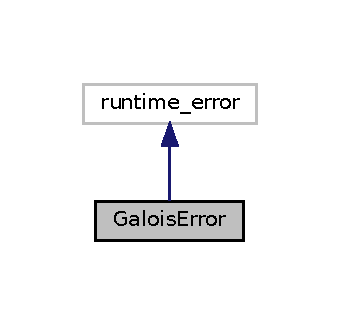
\includegraphics[width=163pt]{classGaloisError__inherit__graph}
\end{center}
\end{figure}


Граф связей класса Galois\+Error\+:
\nopagebreak
\begin{figure}[H]
\begin{center}
\leavevmode
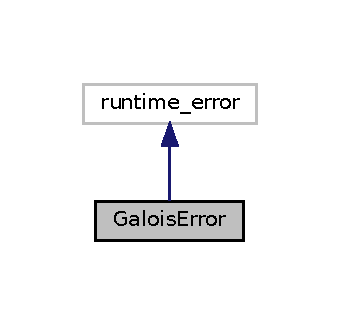
\includegraphics[width=163pt]{classGaloisError__coll__graph}
\end{center}
\end{figure}
\subsection*{Открытые члены}
\begin{DoxyCompactItemize}
\item 
\hyperlink{classGaloisError_a23edc44b479adce2d5d7869d39807575}{Galois\+Error} (const char $\ast$what\+\_\+arg)
\begin{DoxyCompactList}\small\item\em Принимает си строку, поднимает исключение \end{DoxyCompactList}\end{DoxyCompactItemize}


\subsection{Подробное описание}
Класс-\/исключение 

\subsection{Конструктор(ы)}
\mbox{\Hypertarget{classGaloisError_a23edc44b479adce2d5d7869d39807575}\label{classGaloisError_a23edc44b479adce2d5d7869d39807575}} 
\index{Galois\+Error@{Galois\+Error}!Galois\+Error@{Galois\+Error}}
\index{Galois\+Error@{Galois\+Error}!Galois\+Error@{Galois\+Error}}
\subsubsection{\texorpdfstring{Galois\+Error()}{GaloisError()}}
{\footnotesize\ttfamily Galois\+Error\+::\+Galois\+Error (\begin{DoxyParamCaption}\item[{const char $\ast$}]{what\+\_\+arg }\end{DoxyParamCaption})\hspace{0.3cm}{\ttfamily [inline]}, {\ttfamily [explicit]}}



Принимает си строку, поднимает исключение 


\begin{DoxyParams}{Аргументы}
{\em what\+\_\+arg} & \\
\hline
\end{DoxyParams}


Объявления и описания членов класса находятся в файле\+:\begin{DoxyCompactItemize}
\item 
\hyperlink{Galois__LFSR_8h}{Galois\+\_\+\+L\+F\+S\+R.\+h}\end{DoxyCompactItemize}

\chapter{Файлы}
\hypertarget{Galois__LFSR_8cpp}{}\section{Файл Galois\+\_\+\+L\+F\+S\+R.\+cpp}
\label{Galois__LFSR_8cpp}\index{Galois\+\_\+\+L\+F\+S\+R.\+cpp@{Galois\+\_\+\+L\+F\+S\+R.\+cpp}}


Конструктор по-\/умолчанию, не принимает ничего на вход.  


{\ttfamily \#include \char`\"{}Galois\+\_\+\+L\+F\+S\+R.\+h\char`\"{}}\newline
Граф включаемых заголовочных файлов для Galois\+\_\+\+L\+F\+S\+R.\+cpp\+:
\nopagebreak
\begin{figure}[H]
\begin{center}
\leavevmode
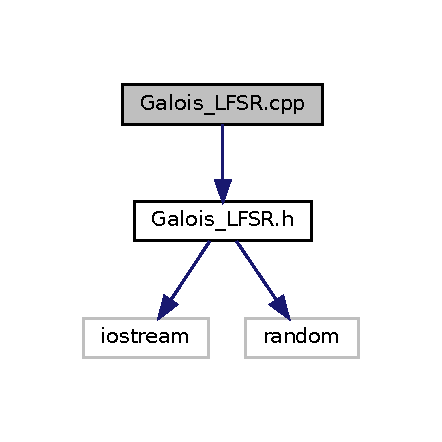
\includegraphics[width=212pt]{Galois__LFSR_8cpp__incl}
\end{center}
\end{figure}


\subsection{Подробное описание}
Конструктор по-\/умолчанию, не принимает ничего на вход. 


\hypertarget{Galois__LFSR_8h}{}\section{Файл Galois\+\_\+\+L\+F\+S\+R.\+h}
\label{Galois__LFSR_8h}\index{Galois\+\_\+\+L\+F\+S\+R.\+h@{Galois\+\_\+\+L\+F\+S\+R.\+h}}


Программа генерации псевдослучайно последовательности на базе регистра сдвига с линейной обратной связью с разрядностью 48 бит в конфигурации Галуа.  


{\ttfamily \#include $<$iostream$>$}\newline
{\ttfamily \#include $<$random$>$}\newline
Граф включаемых заголовочных файлов для Galois\+\_\+\+L\+F\+S\+R.\+h\+:
\nopagebreak
\begin{figure}[H]
\begin{center}
\leavevmode
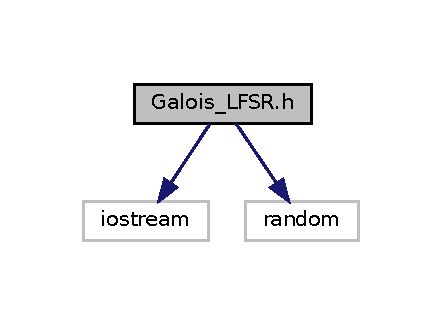
\includegraphics[width=212pt]{Galois__LFSR_8h__incl}
\end{center}
\end{figure}
\subsection*{Классы}
\begin{DoxyCompactItemize}
\item 
class \hyperlink{classGalois__LFSR}{Galois\+\_\+\+L\+F\+SR}
\item 
class \hyperlink{classGaloisError}{Galois\+Error}
\begin{DoxyCompactList}\small\item\em Класс-\/исключение \end{DoxyCompactList}\end{DoxyCompactItemize}


\subsection{Подробное описание}
Программа генерации псевдослучайно последовательности на базе регистра сдвига с линейной обратной связью с разрядностью 48 бит в конфигурации Галуа. 


\hypertarget{main_8cpp}{}\section{Файл main.\+cpp}
\label{main_8cpp}\index{main.\+cpp@{main.\+cpp}}
{\ttfamily \#include $<$stdio.\+h$>$}\newline
{\ttfamily \#include $<$iostream$>$}\newline
{\ttfamily \#include \char`\"{}Galois\+\_\+\+L\+F\+S\+R.\+h\char`\"{}}\newline
Граф включаемых заголовочных файлов для main.\+cpp\+:
\nopagebreak
\begin{figure}[H]
\begin{center}
\leavevmode
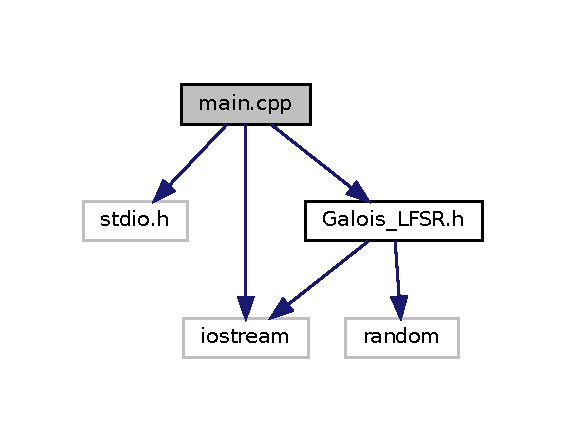
\includegraphics[width=272pt]{main_8cpp__incl}
\end{center}
\end{figure}
\subsection*{Функции}
\begin{DoxyCompactItemize}
\item 
\mbox{\Hypertarget{main_8cpp_a3c04138a5bfe5d72780bb7e82a18e627}\label{main_8cpp_a3c04138a5bfe5d72780bb7e82a18e627}} 
int {\bfseries main} (int argc, char $\ast$$\ast$argv)
\end{DoxyCompactItemize}

%--- End generated contents ---

% Index
\backmatter
\newpage
\phantomsection
\clearemptydoublepage
\addcontentsline{toc}{chapter}{Алфавитный указатель}
\printindex

\end{document}
